\documentclass[a4paper,12pt]{book}
\usepackage[utf8]{inputenc}
\title{}
\author{Rachel Morris}
\date{\today}

\usepackage{rachwidgets}
\usepackage{fancyhdr}
\usepackage{lastpage}
\usepackage{boxedminipage}

\pagestyle{fancy}
\fancyhf{}
\lhead{CS 210}
\chead{Fall 2017}
\rhead{Ch 1.1 Exercise}
\rfoot{\thepage\ of \pageref{LastPage}}
\lfoot{\scriptsize By Rachel Morris, last updated \today}
\newcounter{question}

\renewcommand{\headrulewidth}{2pt}
\renewcommand{\footrulewidth}{1pt}

\begin{document}
    
    %\toggletrue{answerkey}
    \togglefalse{answerkey}

    %------------------------------------------------------------------%
    %- INSTRUCTIONS ---------------------------------------------------%
    %------------------------------------------------------------------%

    \chapter*{Chapter 1.1 In-class Exercise} \stepcounter{chapter}

    \iftoggle{answerkey}{
      \begin{answer} ANSWER KEY \end{answer}
    }{}

    \paragraph{Info:}
    In-class exercises are meant to introduce you to the new topics
    of this chapter of the book. Each part will have an introductory
    description of the content and example(s), followed by practice
    problems for you to work on. ~\\

    These assignments are \textbf{team assignments} - your team will
    turn in \textit{one} copy of the exericse. It is up to your team
    how to appropach the assignments; you can work separately and then
    check your work together, or you can collaborate on the assignment
    together. ~\\

    Work must be clean; points may be deducted if the instructor cannot
    read the work.

    \begin{center}
        \textbf{This is the instruction page, \\
        make sure to fill out your answers to turn in on the worksheet}
    \end{center}
    
    \hrulefill{}
    
    \newpage{}

    %------------------------------------------------------------------%
    %- Exercise Begin -------------------------------------------------%
    %------------------------------------------------------------------%

    %------------------------------------------------------------------%
    \section*{1. Coin toss}

        \begin{intro}{Coin toss}
            When we're flipping a coin, there are two possible outcomes:
            \textit{heads} or \textit{tails}. If we flip more than one
            coin, then we end up with more possible outcomes. For example,
            when flipping two coins, we have four possible outcomes:

            \begin{center}
                \begin{tabular}{ | l | c | c | }
                    \hline
                    1. & HEADS & HEADS \\ \hline
                    2. & HEADS & TAILS \\ \hline
                    3. & TAILS & HEADS \\ \hline
                    4. & TAILS & TAILS \\ \hline
                \end{tabular}
            \end{center}
        \end{intro}

        % - QUESTION --------------------------------------------------%
        \stepcounter{question}
        \begin{questionNOGRADE}{\thequestion}
            Draw a table of all possible outcomes if someone flips three coins.
        \end{questionNOGRADE}

        % - QUESTION --------------------------------------------------%
        \stepcounter{question}
        \begin{questionNOGRADE}{\thequestion}
            Write out how many outcomes there are for each of the following.

            \begin{enumerate}
                \item Flipping one coin
                \item Flipping two coins
                \item Flipping three coins
                \item Rolling one 6-sided die
                \item Rolling two 6-sided dice
                \item Rolling three 6-sided dice
            \end{enumerate}
        \end{questionNOGRADE}

        % - QUESTION --------------------------------------------------%
        \stepcounter{question}
        \begin{questionNOGRADE}{\thequestion}
            So if we have $n$ possible outcomes per event (roll die, flip coin),
            and we ``run" the event $m$ times (one coin, two dice),
            how many total outcomes $ o $ will there be? (Write as a simple equation).
        \end{questionNOGRADE}

    %------------------------------------------------------------------%
    \newpage
    \section*{2. Josephus game}

        \begin{intro}{The Josephus game}
            The Josephus game is a theoretical problem, and for now we
            will just solve it systematically by stepping through the
            instructions given.

            \paragraph{Setup:} People are sitting in a circle, each with
            an assigned number (their location in the circle).

            \paragraph{Step:} People are eliminated at every $n$th step,
            with counting beginning at the $n$th person.

            \paragraph{Result:} After stepping through, figure out the
            position of the \textit{last} and \textit{second-to-last}
            person left (not eliminated).

            \paragraph{Example:} Let's say that we begin with a circle of
            \textit{10} people, numbered from 1 to 10. We will eliminate
            people at an interval of \textit{2} - so, every-other-person,
            beginning with person \#2. Who will be the last person standing?

            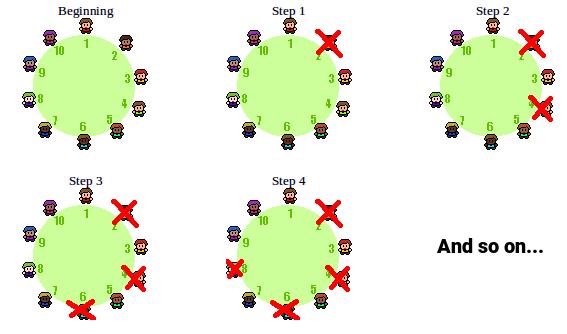
\includegraphics[width=12cm]{images/josephus.png}
        \end{intro}

        \newpage{}
        
        % - QUESTION --------------------------------------------------%
        \stepcounter{question}
        \begin{questionNOGRADE}{\thequestion}
            Given a Josephus circle of 15 people,
            if we are eliminating every 3rd person (starting with person 3),
            who is the last to be ``killed" – and the 2nd to last to be ``killed"?

            \begin{center}
                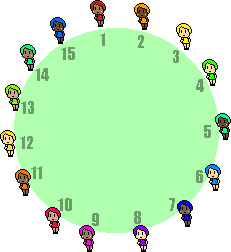
\includegraphics[width=6cm]{images/josephus-15.png}
            \end{center}

            \begin{hint}{Hint:}
                Don't count ``dead" people, make sure to skip over them!
            \end{hint}
            
        \end{questionNOGRADE}

        % - QUESTION --------------------------------------------------%
        \stepcounter{question}
        \begin{questionNOGRADE}{\thequestion}
            Given a Josephus circle of 10 people,
            if we are eliminating every 4th person (starting with person 4),
            who is the last to be ``killed" – and the 2nd to last to be ``killed"?

            \begin{center}
                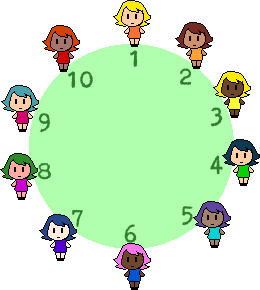
\includegraphics[width=7cm]{images/josephus-10.png}
            \end{center}
        \end{questionNOGRADE}
       
    %------------------------------------------------------------------% 
    \newpage
    \section*{3. Game trees}

        \begin{intro}{Game trees}
            In section 1.1, we will also be looking at events that have multiple outcomes –
            such as flipping one coin, two coins, or three coins, or who of two people win
            one, two, or three tennis matches. With small amounts of ``variables", we can
            list out all the possible outcomes, and we can build a game tree based on this.
            
            \paragraph{Example:} ~\\
            If you flip one coin, the result with be HEADS (H) or TAILS (T).
            If you flip two coins, what are all the outcomes?

            \begin{center}
                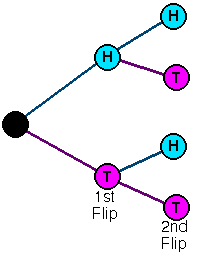
\includegraphics[width=5cm]{images/gametree.png}
                
                \begin{tabular}{l l}
                    1. HH &  2. HT \\
                    3. TH &  4. TT
                \end{tabular}
            \end{center}

        \end{intro}

        \newpage
        % - QUESTION --------------------------------------------------%
        \stepcounter{question}
        \begin{questionNOGRADE}{\thequestion}
            Suppose you toss three coins – a nickel, a dime, and a quarter,
            and you record the results in that order. For example,
            ``HTH" means nickel = heads, dime = tails, quarter = heads.

            \begin{enumerate}
                \item In a systematic way, list all the different results you could record.
                \item Draw a game tree for recording the results.
                \item On the game tree, label each possible result either 0, 1, 2, or 3,
                to indicate how many \textit{heads} there are.
                \item Do you think a person who tosses three coins is more likely to get all
                three heads, or to get exactly two heads?                
            \end{enumerate}
        \end{questionNOGRADE}


    %------------------------------------------------------------------%
    %- WORKSHEET ------------------------------------------------------%
    %------------------------------------------------------------------%
    \newpage
    \begin{center} \section*{Chapter 1.1 In-class Exercise Worksheet} \end{center}

    \iftoggle{answerkey}{
      \begin{answer} \begin{center} ANSWER KEY \end{center} \end{answer}
    }{}

    \paragraph{Team:}
    Please write down all people in your team. ~\\

    % table %
    \begin{tabular}{ p{6cm} p{6cm} }
        1. & 2. \\
        3. & 4.
    \end{tabular}
    % table %
    
    \paragraph{Section:} ~\\
        $\Box$ MW 4:30 - 5:45 pm \tab
        $\Box$ M 6:00 - 8:50 pm \tab
        $\Box$ TR 2:00 - 3:15 pm

    \paragraph{Team rules:}

    \begin{itemize}
        \item \textbf{Only one worksheet will be turned in per team.}
            Each member of the team will receive the same score.
        \item You can collaborate on the exercise together, or you can
            work separately and then compare your answers with your team
            as you fill out the turn-in worksheet.
    \end{itemize}

    \paragraph{Work rules:}

    \begin{itemize}
        \item Fill out your answers on this answer sheet.
        \item Write cleanly and linearly - if I can't make sense of
            your solution then you won't get credit.
        \item Write out each step (within reason) - if I can't see the
            logic you followed to get to your answer, you may get points taken off.
        \item Don't scribble out cancellations - I can't read that.
            For example, if a numerator/denominator cancel out, or a +/-
            cancels out, don't scribble out the numbers - just use a single slash!
    \end{itemize}

    \paragraph{Grading:}
        The total amount of points for an in-class exercise is 5 points each.
        Each question will have a weight assigned to it, and will be given
        a a point value between 0 and 4:

    \begin{center}
        \begin{tabular}{ | l | l | }
            \hline
            0 & Nothing written \\ \hline
            1 & Something written, but incorrect \\ \hline
            2 & Partially correct, but multiple errors \\ \hline
            3 & Mostly correct, with one or two errors \\ \hline
            4 & Perfect; correct answer and notation \\ \hline
            
        \end{tabular}
    \end{center}
    
    \newpage{}

    %------------------------------------------------------------------%
    %- Exercise Begin -------------------------------------------------%
    %------------------------------------------------------------------%

    %------------------------------------------------------------------%
    \section*{Answer sheet}

    \begin{questionNOGRADE}{1}{Draw a table of 3 coins tossed}{10}
        \iftoggle{answerkey}{ \begin{answer}
            \begin{center}
                \begin{tabular}{ | l | c | c | c | }
                    \hline
                    1. & HEADS & HEADS & HEADS \\ \hline
                    2. & HEADS & HEADS & tails \\ \hline
                    3. & HEADS & tails & HEADS \\ \hline
                    4. & HEADS & tails & tails \\ \hline
                    5. & tails & HEADS & HEADS \\ \hline
                    6. & tails & HEADS & tails \\ \hline
                    7. & tails & tails & HEADS \\ \hline
                    8. & tails & tails & tails \\ \hline
                \end{tabular}
            \end{center}
        \end{answer} }{ ~\\ \raisebox{0pt}[4cm][0pt]{  } }
    \end{questionNOGRADE}

    ~\\ \begin{questionNOGRADE}{2}{How many outcomes?}{30}
        \begin{enumerate}
            \item Flipping one coin: \fitb{}            \iftoggle{answerkey}{\begin{answer} ($2^{1} = 2$) \end{answer} } {}
            \item Flipping two coins: \fitb{}           \iftoggle{answerkey}{\begin{answer} ($2^{2} = 4$) \end{answer} } {}
            \item Flipping three coins: \fitb{}         \iftoggle{answerkey}{\begin{answer} ($2^{3} = 8$) \end{answer} } {}
            
            \item Rolling one 6-sided die: \fitb{}      \iftoggle{answerkey}{\begin{answer} ($6^{1} = 6$) \end{answer} } {}
            \item Rolling two 6-sided dice: \fitb{}     \iftoggle{answerkey}{\begin{answer} ($6^{2} = 36$) \end{answer} } {}
            \item Rolling three 6-sided dice: \fitb{}   \iftoggle{answerkey}{\begin{answer} ($6^{3} = 216$) \end{answer} } {}
        \end{enumerate}
    \end{questionNOGRADE}


    ~\\
    \begin{questionNOGRADE}{3}{Equation for outcomes}{10}
        $ o = $ \iftoggle{answerkey}{\begin{answer} $ n^{m} $ \end{answer} } {}
    \end{questionNOGRADE}

    
    ~\\
    \begin{questionNOGRADE}{4}{Jospehus game A}{10}
        {2nd-to-last:} \fitb    \iftoggle{answerkey}{ \begin{answer} Person 14 \end{answer} }{}
        {Last:} \fitb          \iftoggle{answerkey}{ \begin{answer} Person 5 \end{answer} }{}
    \end{questionNOGRADE}

    
    ~\\
    \begin{questionNOGRADE}{5}{Jospehus game B}{10}
        {2nd-to-last:} \fitb    \iftoggle{answerkey}{ \begin{answer} Person 6 \end{answer} }{}
        {Last:} \fitb          \iftoggle{answerkey}{ \begin{answer} Person 5 \end{answer} }{}
        
    \end{questionNOGRADE}

    
    ~\\
    \newpage
    \begin{questionNOGRADE}{6}{Game tree}{30}
        \begin{enumerate}
            \item In a systematic way, list all the different results you could record.

            \iftoggle{answerkey}{ \begin{answer} 1. HHH, 2. HHT, 3. HTH, 4. HTT, \\ 5. THH, 6. THT, 7. TTH, 8. TTT
            \end{answer} }{ { ~\\ \raisebox{0pt}[2cm][0pt]{  } } }

            \item Draw a game tree for recording the results

            \iftoggle{answerkey}{ \begin{answer}

            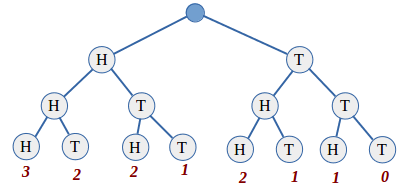
\includegraphics[width=6cm]{images/ans-gametree.png}
            
            \end{answer} }{ { ~\\ \raisebox{0pt}[6cm][0pt]{  } } }

            \item On the game tree, label each possible result either 0, 1, 2, or 3,
            to indicate how many \textit{heads} there are.

            \item Do you think a person who tosses three coins is more likely to get all
            three heads, or to get exactly two heads?
            
            \iftoggle{answerkey}{ \begin{answer} More likely to get exactly 2 heads \end{answer} }{}
            
        \end{enumerate}
    \end{questionNOGRADE}


    %------------------------------------------------------------------%
    %- Grading --------------------------------------------------------%
    %------------------------------------------------------------------%
    \hrulefill{}
    \subsection*{Grading}
    
    \begin{center}
        
        \begin{tabular}{ | l | l | l | l | }
            \hline
            \textbf{ Question } & \textbf{ Weight } & \textbf{ 0-4 } & \textbf{ Adjusted score }
            \\ \hline{}
            
            1 & 10\% & &    \\ \hline
            2 & 30\% & &    \\ \hline
            3 & 10\% & &    \\ \hline
            4 & 10\% & &    \\ \hline
            5 & 10\% & &    \\ \hline
            6 & 30\% & &    \\ \hline
            & & & \\ \hline
            & & & \\ \hline
            
            
        \end{tabular}
    \end{center}

\end{document}
